\section{Ejercicio III: Heur\'istica de b\'usqueda local}

\subsection{Introducci\'on}
\label{sec:ej3_intro}

B\'usqueda local es un m\'etodo que parte de una soluci\'on no \'optima a un problema e intenta mejorarla a trav\'es de modificaciones, es decir, convirti\'endola en una soluci\'on \textit{vecina}. Luego, es necesario determinar qu\'e constituye una soluci\'on vecina a otra dada, hay que definir un \textit{vecindario}. Por ejemplo, en nuestro problema a resolver, donde una soluci\'on s* es un camino simple, que cumple ciertas condiciones, entre algunos nodos de un grafo, una soluci\'on vecina s a s* podr\'ia ser un camino id\'entico al de s* excepto por un nodo n que se reemplaza con otro n' que s* no recorre. Donde el reemplazo se interpreta como avanzar en s desde el predecesor de n en s* hacia n' y luego continuar por el siguiente de n en s*.

Presentamos a continuaci\'on un pseudoc\'odigo que ilustra la idea general de este algoritmo, en \'el asumimos que queremos minimizar f(s) donde s es una soluci\'on y f una funci\'on que la eval\'ua.

\begin{algorithm}[H]
\label{}
\caption{Idea general de b\'usqueda local}
\begin{algorithmic}[1]
\Statex \underline{Entrada}: S un conjunto de soluciones, N una funci\'on que devuelve las soluciones vecinas a otra dada y f una funci\'on que eval\'ua una soluci\'on
\medskip
\State s* $\gets$ s $\in$ S
\While{($\exists$ s $\in$ N(s*)) f(s) $<$ f(s*)}
    \State s* $\gets$ s $\in$ N(s*) tal que f(s) $<$ f(s*)
\EndWhile
\medskip
\Statex \underline{Salida}: s*
\end{algorithmic}
\end{algorithm}

\subsection{Algoritmo}

Para implementar una heur\'istica de b\'usqueda local para nuestro problema utilizamos una clase llamada \texttt{Camino} que est\'a formada por un grafo (en nuestra implementaci\'on son instancias de la clase \texttt{Grafo}), el tamaño de la mochila, la distancia computada hasta el momento y un puntero al primer nodo del grafo visitado en el recorrido actual, siendo todos los nodos elementos del tipo \texttt{Nodo}.

La clase \texttt{Grafo} est\'a compuesta por un vector de nodos y una matriz con la distancia entre cada par de nodos. Esta distancia se corresponde con la distancia euclideana\footnote{\url{https://es.wikipedia.org/wiki/Distancia_euclidiana}} calculada utilizando sus coordenadas.

Cada instancia de \texttt{Nodo} tiene un n\'umero de identificaci\'on, sus coordendas x e y, la cantidad de pociones que demanda u otorga, un valor booleano que indica si el nodo representa a un gimnasio, un puntero a su nodo anterior y otro a su nodo siguiente dentro del camino actual.

Luego, utilizando las estructuras descriptas anteriormente, realizamos una implementaci\'on que \textit{soporta} dos criterios distintos de vecindad:

\paragraph{Vecindad I: Permutaci\'on del camino}
Establecemos que s* es una soluci\'on vecina a s si el camino de s* se puede obtener permutando el orden en el que se recorren dos nodos en s. Este criterio se conoce comunmente como \textit{swap}.

\paragraph{Vecindad II: Permutaci\'on y reemplazo de las pokeparadas}
Este vecindario considera que s* es una soluci\'on vecina a otra s si el camino de s* es igual al de s luego de permutar el orden en el que se recorren dos pokeparadas, o reemplazar una pokeparada del camino por otra que no se encontraba en \'el. La motivaci\'on principal de esta vecindad fue suponer que una heur\'istica golosa podr\'ia encontrar un buen camino entre los gimnasios pero tendr\'ia dificultades estableciendo los \textit{desv\'ios} para buscar pociones.

\paragraph{}
Como explicamos en la secci\'on \ref{sec:ej3_intro}, para realizar una b\'usqueda local tomamos una soluci\'on inicial que luego es \textit{mejorada}. Para esto decidimos utilizar el algoritmo goloso desarrollado en el segundo ejercicio.

Adem\'as, optamos por considerar tambi\'en las soluciones que devuelven una misma distancia final cuando no podemos encontrar soluciones vecinas que reduzcan ese n\'umero. Esperamos que en algunos casos esto nos permita hallar mejoras nuevas. Para evitar entrar en ciclos infinitos, por ejemplo, donde vamos de una soluci\'on s* a otra s equivalente, y de ella nuevamente volvemos a s*, utilizamos un diccionario donde tenemos como clave la identificaci\'on de un nodo y como significado un conjunto con las identificaciones de los nodos que fueron permutados o reemplazados por el primero. De esta manera tambi\'en limitamos la cantidad de soluciones equivalentes para analizar.

Todo lo descripto anteriormente se encuentra resumido en el siguiente pseudoc\'odigo:

\begin{algorithm}[H]
\label{}
\caption{B\'usqueda local}
\begin{algorithmic}[1]
\Statex \underline{Entrada}: camino : \texttt{Camino} y criterio : \texttt{Vecindad}
\medskip
\State camino.asignarSoluci\'onGolosa()
\If{camino.encontr\'eCamino()}
    \If{criterio == permutaCamino}
        \State nodosConsiderados $\gets$ nodos que forman el camino hallado por el algoritmo goloso
    \Else
        \State nodosConsiderados $\gets$ nodos que representan a las pokeparadas del grafo
    \EndIf
    \State busco $\gets$ true
    \State dicc(int, conj(int)) nodosCambiados $\gets$ Vac\'io()
    \While{busco}
        \While{camino.encuentroSoluci\'onVecinaMejor(nodosConsiderados)}
            \If{\#nodosCambiados.claves() $>$ 0}
                \State nodosCambiados $\gets$ Vac\'io()
            \EndIf
        \EndWhile
        \If{$\neg$camino.encuentroSoluci\'onVecinaIgual(nodosConsiderados, nodosCambiados)}
            \State busco $\gets$ false
        \EndIf
    \EndWhile
\EndIf
\medskip
\Statex \underline{Salida}: camino.imprimirSoluci\'on()
\end{algorithmic}
\end{algorithm}

Como podemos observar en las l\'ineas 12 y 13, si encuentro una soluci\'on que mejora la que ten\'ia vac\'io el diccionario por si ven\'ia de modificar mi camino por otro de distancia igual. Los ciclos \'unicamente ocurren cuando recorro soluciones equivalentes entre si.

Es importante destacar que la funci\'on \texttt{encuentroSoluci\'onVecinaMejor} devuelve el valor booleano \texttt{true} si encuentra una, y realiza las modificaciones necesarias en la instancia de \texttt{Camino} para transformar la soluci\'on actual en la vecina hallada. Como el comportamiento de \texttt{encuentroSoluci\'onVecinaIgual} es an\'alogo, sumando la consulta al diccionario que recibe como argumento para evitar ciclos, exihibimos \'unicamente un psuedoc\'odigo de \texttt{encuentroSoluci\'onVecinaMejor}:

\begin{algorithm}[H]
\label{}
\caption{Encuentro una soluci\'on vecina mejor}
\begin{algorithmic}[1]
\Statex \underline{Entrada}: nodosConsiderados : \texttt{vector(Nodo)}
\medskip
\State busco $\gets$ true
\For{i = 0, ..., nodosConsiderados.tamaño()}
    \For{j = 0, ..., nodosConsiderados.tamaño()}
        \If{i $\neq$ j $\land$ (est\'aEnElCamino(nodosConsiderados[i]) $\lor$ est\'aEnElCamino(nodosConsiderados[j])) $\land$ cambiarMejora(nodosConsiderados[i], nodosConsiderados[j]))}
            \State busco $\gets$ false
        \EndIf
    \EndFor
\EndFor
\medskip
\Statex \underline{Salida}: $\neg$busco
\end{algorithmic}
\end{algorithm}

En s\'intesis, el algoritmo anterior toma cada par de nodos perteneciente al vector recibido y, apenas encuentra un par con un elemento que est\'a en el camino actual y que permite mejorar la distancia actual con su reemplazo o permutaci\'on, realiza la modificaci\'on, si esta fuera posible, y devuelve \texttt{true}. Que uno de los nodos no est\'e en el camino actual significa que mis nodos considerados son pokeparadas y estoy contemplando hacer un reemplazo, sino es una permutaci\'on del camino. \texttt{cambiarMejora} eval\'ua la distancia nueva luego de la modificaci\'on, si es menor a la actual y el cambio es posible, lo realiza y retorna \texttt{true}.

\begin{figure}[H]
  \begin{center}
    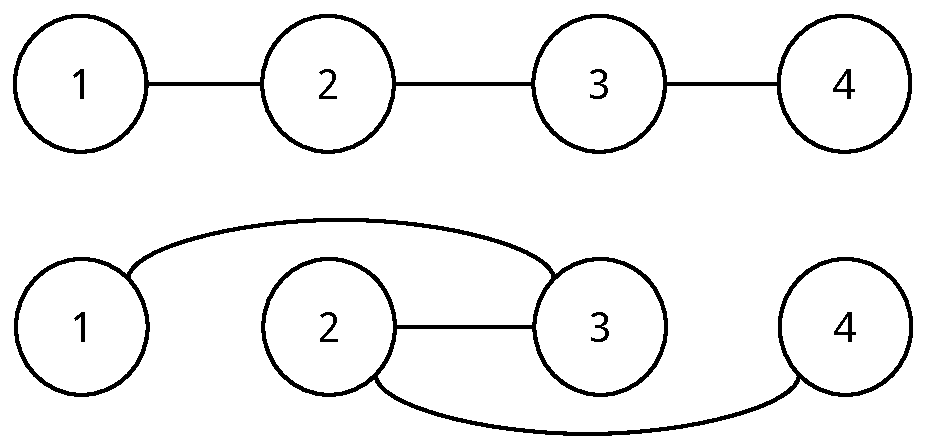
\includegraphics[scale = 0.5]{imagenes/ej3_algoritmo_1.pdf}
    \caption{Permutaci\'on de los nodos 2 y 3 en un camino posible del grafo.}
    \label{fig:ej3_algoritmo_1}
  \end{center}
\end{figure}

Para calcular la distancia nueva utilizamos los punteros almacenados en cada nodo. Si, por ejemplo, estuvi\'eramos en el caso de la figura \ref{fig:ej3_algoritmo_1} el c\'alculo realizado ser\'ia:
\begin{equation*}
    distancia\ nueva = distancia\ actual - distancia(1,2) - distancia(3,4) + distancia(1,3) + distancia(2,4)
\end{equation*}

\begin{figure}[H]
  \begin{center}
    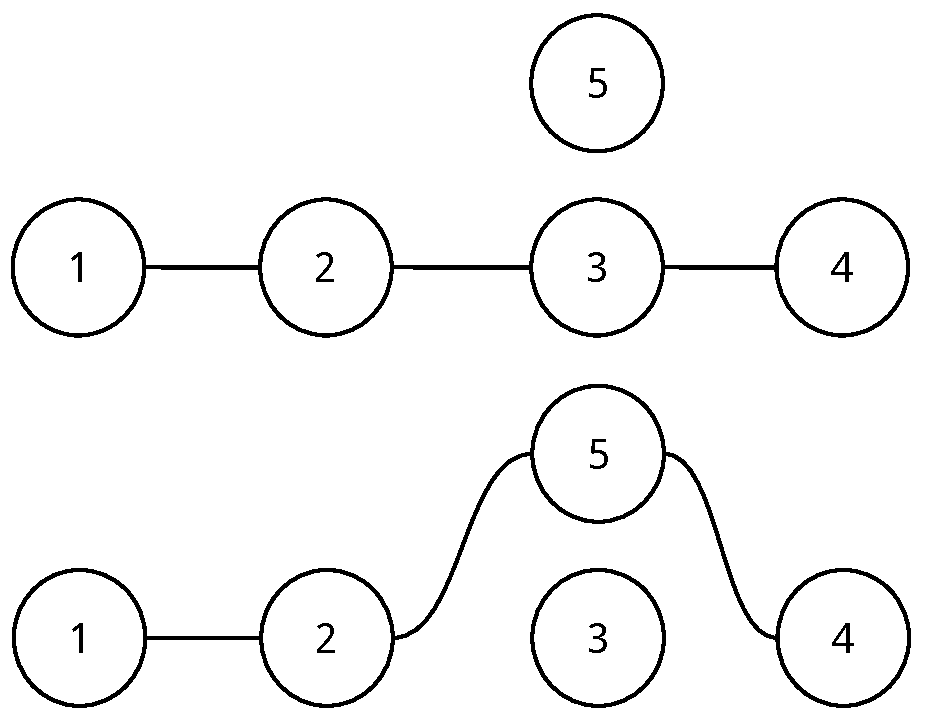
\includegraphics[scale = 0.5]{imagenes/ej3_algoritmo_2.pdf}
    \caption{Reemplazo del nodo 3 por el 5 en un camino posible del grafo.}
    \label{fig:ej3_algoritmo_2}
  \end{center}
\end{figure}

Si la modificaci\'on fuera un reemplazo, como, por ejemplo, en la figura \ref{fig:ej3_algoritmo_2}:
\begin{equation*}
    distancia\ nueva = distancia\ actual - distancia(2,3) - distancia(3,4) + distancia(2,5) + distancia(5,4)
\end{equation*}

Analizamos si el reemplazo o la permutaci\'on es posible teniendo en cuenta las pociones que requieren los gimnasios, las que otorgan las pokeparadas y la capacidad de nuestra mochila. Con este fin avanzamos desde el nodo inicial de nuestra instancia de \texttt{Camino}, llevando la cuenta de cu\'antas pociones tenemos en nuestra mochila. Si el nodo actual es una pokeparada sumamos el m\'inimo entre 3 y lo que le reste de espacio a la mochila, en caso contrario restamos el costo del gimnasio. Si nuestra mochila queda con pociones negativas significa que el cambio no es posible y paramos de iterar, si no continuamos hasta llegar al final del camino. Llegar al nodo que no tiene siguiente significa que el cambio es posible.

\subsection{Complejidad}

El orden de complejidad temporal de peor caso para una iteraci\'on de la b\'usqueda local que mejora una soluci\'on, es decir, para encontrar una soluci\'on vecina s a s* tal que f(s) $<$ f(s*), es \bigo{k^2 \times $tamaño del camino$}, siendo k el tamaño de \texttt{nodosConsiderados}. En la primer vecindad esta complejidad es equivalente a \bigo{($tamaño del camino$)^3} $\in$ \bigo{(n+m)^3} siendo n la cantidad de gimnasios y m la cantidad de pokeparadas. Mientras que la complejidad de la vecindad que permuta y reemplaza pokeparadas es \bigo{m^2 \times $tamaño del camino$} $\in$ \bigo{m^2 \times (n+m)}.

Este tipo de iteraci\'on se corresponde con una ejecuci\'on de \texttt{encuentroSoluci\'onVecinaMejor}, all\'i para cada par de los elementos que componen \texttt{nodosConsiderados} evaluamos si realizar la modificaci\'on nos permite hallar una soluci\'on vecina mejor. En el peor caso no encontramos una hasta la \'ultima iteraci\'on del primer ciclo, es decir, realizamos $k^2$ iteraciones. En cada una de las iteraciones realizamos una llamada a \texttt{cambiarMejora} donde se calcula la distancia nueva con una cantidad constante de operaciones \bigo{1}. Si es menor a la distancia actual analiza si el cambio es posible con un costo de \bigo{$tamaño del camino$} $\in$ \bigo{n+m} en el pero caso, cuando el cambio es posible y recorre el camino completo sin obtener una cantidad \textit{negativa} de pociones. Por otra parte, el costo de \texttt{est\'aEnElCamino} es \bigo{1} porque simplemente revisa que los atributos \texttt{anterior} y \texttt{siguiente} del nodo no sean ambos inv\'alidos. El costo de realizar efectivamente el reemplazo o la permutaci\'on es \bigo{1} porque tambi\'en \'unicamente altera los atributos \texttt{anterior} y \texttt{siguiente} de los nodos a modificar, y los de sus dos vecinos.

Por otro lado, el orden de complejdidad de peor caso para una iteraci\'on de la b\'usqueda local que encuentra una soluci\'on vecina equivalente es \bigo{(n+m)^3 \times log(n+m)} en la vecindad que \'unicamente permuta y \bigo{m^2 \times (n+m) \times log(n+m)} en la restante.

En este caso una iteraci\'on de la b\'usqueda local se corresponde con una ejecuci\'on de \texttt{encuentro\\ Soluci\'onVecinaIgual}. Como explicamos anteriormente, es equivalente al algoritmo ya descripto, la \'unica diferencia recide en la guarda del \texttt{if}, para evitar ciclos en este caso tambi\'en revisa que nodosConsiderados[j].id $\notin$ nodosCambiados.significado(nodosConsiderados[i].id). En la implementaci\'on utilizamos el m\'etodo \texttt{count} de la clase \texttt{map} y el de la clase \texttt{set}, contenidas en la Standard Template Library de C++, para comprobar si nodosConsiderados[i] est\'a definido en nodosCambiados y luego si nodosConsiderados[j] est\'a contenido en su significado. Ambas operaciones tienen un costo logar\'itmico en funci\'on del tamaño del contenedor\footnote{\url{http://www.cplusplus.com/reference/map/map/count/} y \url{http://www.cplusplus.com/reference/set/set/count/}}. El diccionario tiene como m\'aximo k claves y sus significados en el peor caso son conjuntos de cardinal k.

Ejecutar nuestro algoritmo de b\'usqueda local sobre una soluci\'on inicial produce una cantidad de iteraciones de ambos tipos que no podemos estimar te\'oricamente. En pr\'oxima secci\'on intentamos encontrar una relaci\'on entre el n\'umero de iteraciones y los par\'ametros que recibe nuestro programa.

\subsection{Experimentación}

% ESTE TP: Realizar una experimentacion que permita observar la performance del algoritmo comparando
% los tiempos de ejecucion y la calidad de las soluciones obtenidas, en funci ́on de las vecindadeS utilizadas y elegir, si es posible, la configuraci ́on que mejores resultados provea para el grupo de instancias utilizado.Si es posible, dar una cota superior para la cantidad de iteraciones de la heur ́ıstica.

\subsubsection{Instancias estudiadas}

Con el objetivo de estudiar los algoritmos propuestos realizamos mediciones con diversos tipos de instancias que permiten hallar una soluci\'on por medio de la heur\'istica golosa que estudiamos anteriormente.

En cada medici\'on registramos: la cantidad de gimnasios, la cantidad de pokeparadas, el tamaño de la mochila, la distancia obtenida con la soluci\'on golosa, la distancia mejorada con una b\'usqueda local, la cantidad de permutaciones realizadas para mejorar la soluci\'on actual, la cantidad de permutaciones para cambiar la soluci\'on actual por otra igualmente buena, la cantidad de reemplazos para mejorar la soluci\'on actual, la cantidad de reemplazos para cambiar la soluci\'on actual por otra igualmente buena, el tamaño final del camino y el tiempo demorado en ciclos de reloj.

Para cada tipo creamos una cantidad fija de instancias de \texttt{Camino} y ejecutamos el algoritmo 100 veces. Cuando intentamos comparar nuestras soluciones con el \'optimo obtenido con backtracking ejecutamos este algoritmo 10 veces.

\paragraph{Instancias aleatorias}
Para generar cada instancia elegimos un n\'umero aleatorio de gimnasios entre 1 y 100. A cada gimnasio se le fij\'o una cantidad de pociones entre 0 y 10. Luego, sumamos las pociones que fueron asignadas a todos los gimnasios y elegimos una cantidad de pokeparadas random entre (cantidad total de pociones / 3) + 1 y ((cantidad total de pociones / 3) + 1) $\times$ 2. Las coordenadas de las pokeparadas y de los gimnasios se eligieron como n\'umeros aleatorios entre 0 y 1000. El tamaño de la mochila se determin\'o en 12 para evitar el desperdicio de pociones, debido a que lo m\'aximo que puede requerir un gimnasio es 10 pociones. Para estudiar este tipo creamos 30 instancias.

\paragraph{Instancias aleatorias y sus soluciones \'optimas}
Creamos 18 instancias con 1, 2, ..., 17 y 18 nodos cada una. En cada una elegimos la cantidad de gimnasios como el m\'inimo entre un n\'umero aleatorio entre 1 y la cantidad de nodos, y 10. Los nodos restantes corresponden a pokeparadas. Luego, establecemos que la cantidad m\'axima de pociones que puede pedir un gimnasio es (cantidad de pokeparadas $\times$ 3) / cantidad de gimnasios, y a cada nodo de tipo gimnasio le asignamos una cantidad de pociones aleatoria entre 1 y el m\'inimo entre 10 y el m\'aximo calculado para la instancia. Nuevamente, las coordenadas se eligieron aleatoriamente entre 0 y 1000, y el tamaño de la mochila se fij\'o en 12. Elegimos estas cantidades de 
gimnasios y pokeparadas para poder ejecutar el algoritmo de backtracking sobre estas instancias en un tiempo razonable.

\paragraph{Instancias de mejor caso}
Esperamos que la heur\'istica golosa tenga grandes dificultades para hallar caminos cercanos al \'optimo cuando los gimnasios y las pokeparadas se encuentran en \'areas distintas, ya que en primer lugar busca un camino entre los gimnasios y luego recorre las pokeparadas, lo que causar\'ia una ida y vuelta constante entre ambas \'areas. Estos casos, que podr\'iamos considerar como los \textit{peores} de la heur\'istica golosa, se corresonden con unos de los \textit{mejores} de la b\'usqueda local. Es decir, la b\'usqueda local va a tener un porcentaje de mejora mucho mayor que en instancias aleatorias. Para generarlas procedemos de forma an\'aloga que con las aleatorias, la \'unica diferencia es que los gimnasios ahora tienen como coordenadas n\'umeros entre 0 y 500, y las pokeparadas entre 500 y 1000. Adem\'as, el tamaño de la mochila se elige como la cantidad total de pociones que requieren los gimnasios, lo que permite recorrer primero el \'area de pokeparadas y luego el \'area de gimnasios. Nuevamente, generamos 30 instancias de este tipo.

\paragraph{Instancias de mejor caso y sus soluciones \'optimas}
Con el objetivo de generar este tipo de instancias procedemos de forma an\'aloga a los \'ultimos dos tipos descriptos. Separamos los gimnasios de las pokeparadas y generamos grafos de pocos nodos para poder ejecutar el algoritmo de backtracking.

\paragraph{Instancias con \#gimnasios fija e instancias con \#pokeparadas fija}
En este caso a la variable fija se le asigna el n\'umero 10 y para la restante se elije aleatoriamente otro entre 1 y 100, el tamaño de la mochila es 12 otra vez y creamos 30 instancias. Para determinar la cantidad de pociones que requieren los gimnasios hacemos lo mismo que cuando queremos estudiar soluciones \'optimas y generamos los caminos con un n\'umero fijo de gimnasios y pokeparadas.

\subsubsection{Complejidades}

Para comprobar emp\'iricamente las complejidades te\'oricas dividimos el tiempo de ejecuci\'on por la complejidad respectiva esperando encontrar una funci\'on constante. Estos datos se pueden apreciar con mayor claridad utilizando un \textit{boxplot} con su respectiva densidad:

\begin{figure}[H]
  \begin{center}
    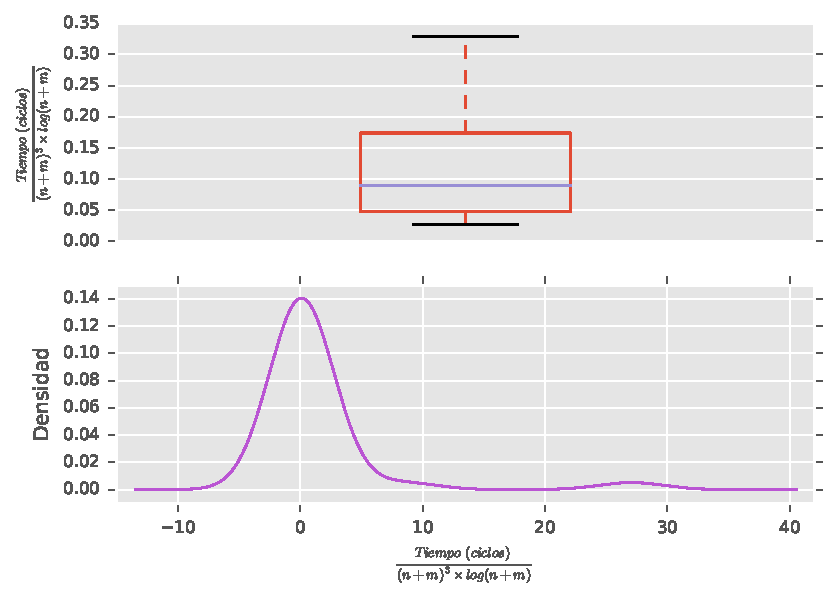
\includegraphics{../experimentacion/ej3/expAleat_complejidad_permutaCamino.pdf}
    \caption{Tiempo sobre complejidad en funci\'on de la cantidad de nodos para la vecindad que permuta el camino, utilizando instancias aleatorias.}
    \label{fig:expAleat_complejidad_permutaCamino}
  \end{center}
\end{figure}

\begin{figure}[H]
  \begin{center}
    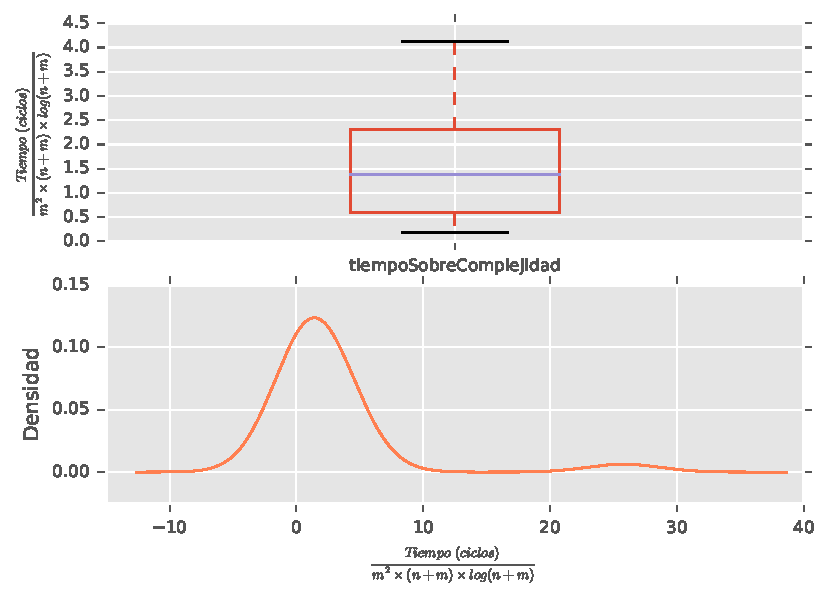
\includegraphics{../experimentacion/ej3/expFijo_complejidad_permutaYReemplazaPokeparadas_cantGimFija.pdf}
    \caption{Tiempo sobre complejidad en funci\'on de la cantidad de nodos para la vecindad que permuta y reemplaza pokeparadas, utilizando una cantidad de gimnasios fija.}
    \label{fig:expFijo_complejidad_permutaYReemplazaPokeparadas_cantGimFija}
  \end{center}
\end{figure}

\begin{figure}[H]
  \begin{center}
    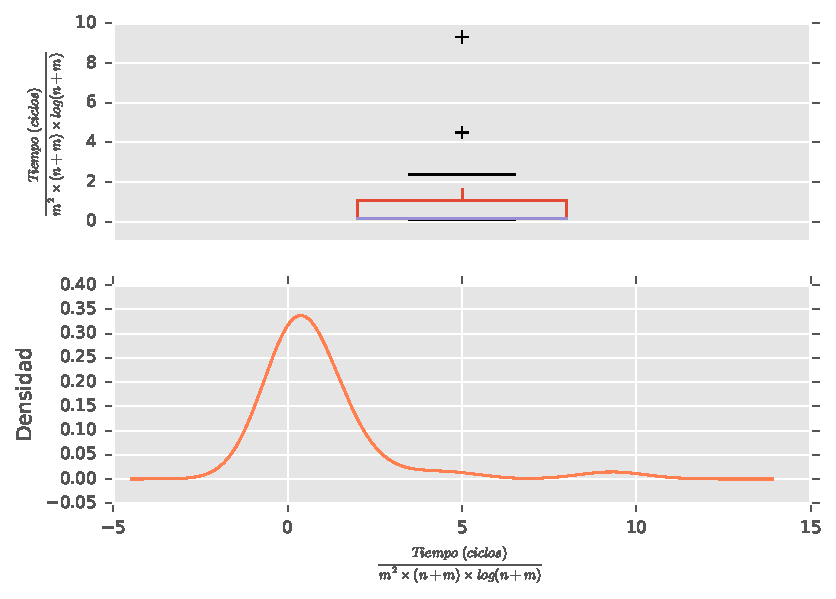
\includegraphics{../experimentacion/ej3/expFijo_complejidad_permutaYReemplazaPokeparadas_cantPokFija.pdf}
    \caption{Tiempo sobre complejidad en funci\'on de la cantidad de nodos para la vecindad que permuta y reemplaza pokeparadas, utilizando una cantidad de pokeparadas fija.}
    \label{fig:expFijo_complejidad_permutaYReemplazaPokeparadas_cantPokFija}
  \end{center}
\end{figure}

Como podemos observar en las figuras \ref{fig:expAleat_complejidad_permutaCamino}, \ref{fig:expFijo_complejidad_permutaYReemplazaPokeparadas_cantGimFija} y \ref{fig:expFijo_complejidad_permutaYReemplazaPokeparadas_cantPokFija} la relaci\'on entre el tiempo de ejecuci\'on y las cotas te\'oricas de los algoritmos es constante, lo que permite dar por \textit{comprobadas} las complejidades.

\subsubsection{\#iteraciones de la b\'usqueda}

Con el objetivo de dar una cota superior para la cantidad de iteraciones que realiza la heur\'istica, es decir, la cantidad de veces que cambia la soluci\'on por otra vecina evaluamos su relaci\'on con la cantidad de nodos del grafo. Nuestra hip\'otesis es que ambas variable tienen una relaci\'on lineal, por lo tanto, al dividirlas deber\'iamos poder observar un valor constante en los gr\'aficos.

\begin{figure}[H]
  \begin{center}
    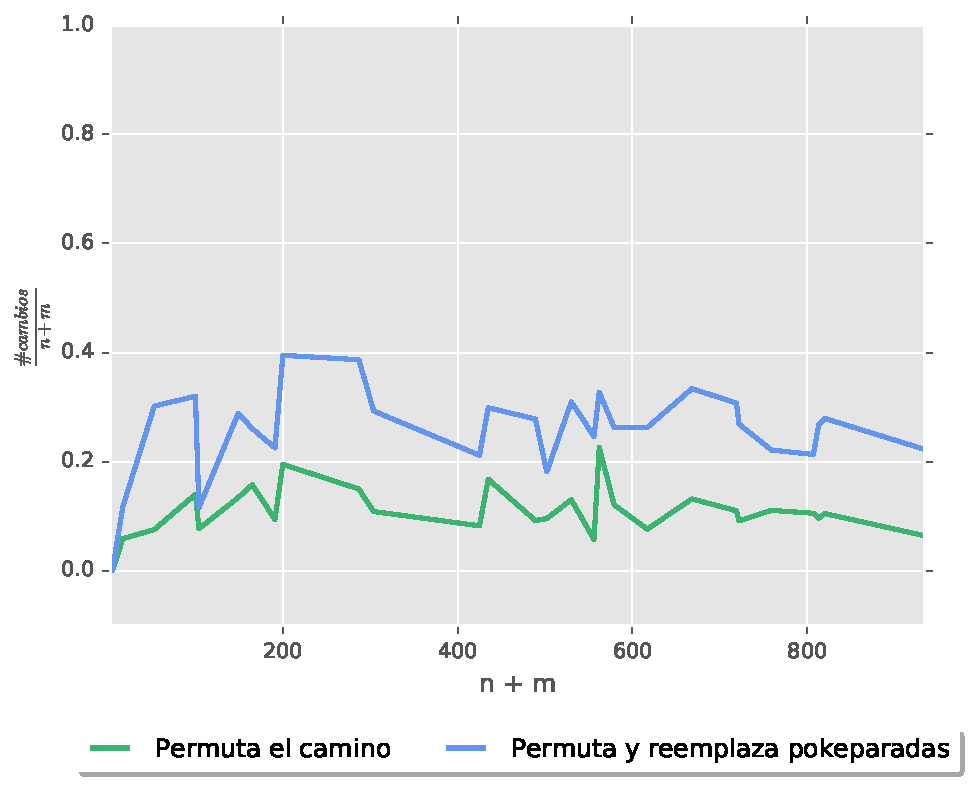
\includegraphics{../experimentacion/ej3/expAleat_cantCambios.pdf}
    \caption{Cantidad de cambios sobre cantidad de nodos en funci\'on de la cantidad de nodos usando instancias aleatorias.}
    \label{fig:expAleat_cantCambios}
  \end{center}
\end{figure}

\begin{figure}[H]
  \begin{center}
    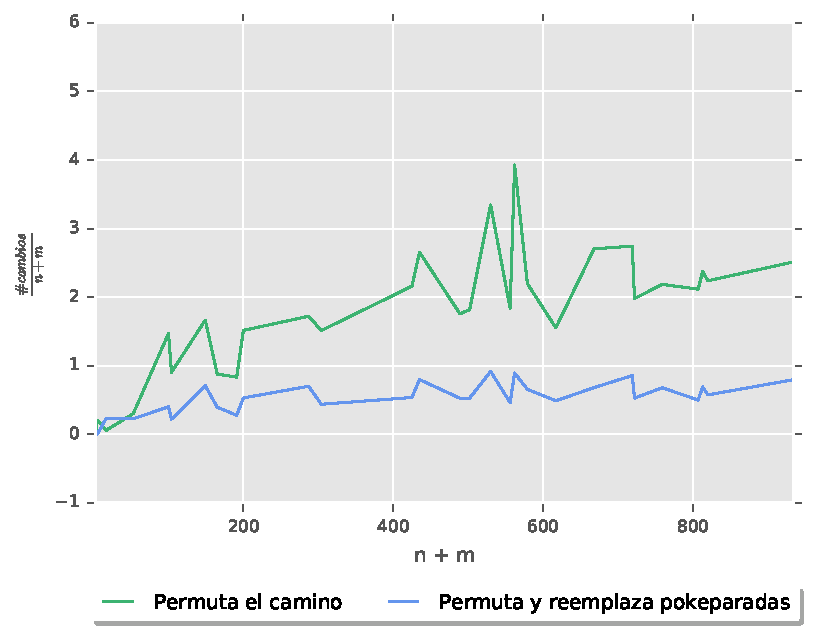
\includegraphics{../experimentacion/ej3/expMejor_cantCambios.pdf}
    \caption{Cantidad de cambios sobre cantidad de nodos en funci\'on de la cantidad de nodos usando instancias de mejor caso para la b\'usqueda.}
    \label{fig:expMejor_cantCambios}
  \end{center}
\end{figure}

En las figuras \ref{fig:expAleat_cantCambios} y \ref{fig:expMejor_cantCambios} no parece haber una pendiente marcada en ning\'un sentido, por lo que podr\'iamos pensar que nuestra hip\'otesis es v\'alida.

Observando el gr\'afico correspondiente a las instancias aleatorias podr\'iamos atrevernos a acotar la cantidad de cambios por n + m, sin embargo, en el mejor caso de la b\'usqueda estos ascienden a 4 $\times$ (n + m). Si este caso es efectivamente el que logra la mayor \textit{mejora} con respecto a la soluci\'on golosa, podr\'ia tambi\'en ser el que m\'as cambios demanda, lo que permitir\'ia acotar la cantidad de iteraciones por 4 $\times$ (n + m).


\subsubsection{Calidad de las soluciones}

El prop\'osito de esta secci\'on es evaluar ambas vecindades en cuanto a la calidad de la soluci\'on, en particular, cu\'anto mejora la distancia original recibida del algoritmo goloso, el costo en tiempo del algoritmo y el error relativo con respecto a la soluci\'on \'optima.

Definimos el porcentaje de mejora de la siguiente manera:

\begin{equation*}
    porcentaje\ de\ mejora = 100 - \frac{distancia\ nueva \times 100}{distancia\ original}
\end{equation*}

Utilizamos esta m\'etrica para evaluar todas las mediciones realizadas con instancias aleatorias y de mejor caso. Esperamos ver una gran diferencia entre ambos tipos, ya que, como mencionamos antes, el algoritmo goloso es especialmente ineficiente cuando las pokeparadas y los gimnasios est\'an esperados. Exihibimos estos datos en el cuadro \ref{table:porcentaje_mejora}.

\begin{table}[H]
    \begin{center}
        \begin{tabular}{ | l | l | l | l | l | }
            \hline
            \multicolumn{1}{|c|}{}&
            \multicolumn{2}{|c|}{\textbf{Instancias aleatorias}}&
            \multicolumn{2}{|c|}{\textbf{Instancias de mejor caso}}\\
            \cline{2-5}
                            &    \textit{Vecindad I}     &    \textit{Vecindad II}    &    \textit{Vecindad I}     &    \textit{Vecindad II}    \\ \hline
            Media           &    11.368223  &   21.943365   &   70.201509   &    8.155963   \\ \hline
            Desv\'io estandar       &   3.848846    &    6.707769   &   20.632809   &   3.791787    \\ \hline
            M\'inimo        &   0.000000    &    0.000000   &   0.000000    &   0.000000    \\ \hline
            M\'aximo        &   18.463784   &    28.902765  &       84.686633   &    23.047859  \\ \hline
        \end{tabular}
    \end{center}
    \caption{Porcentaje de mejora para cada vecindad con instancias aleatorias y de mejor caso. \textit{Vecindad I} es \textit{swap} y \textit{Vecindad II} la restante.}    
    \label{table:porcentaje_mejora}
\end{table} 

Como esper\'abamos, la media del porcentaje var\'ia enormemente. Adem\'as es interesante notar que, como podr\'ia pensarse intuitivamente, la segunda vecindad es superior a la primera en instancias aleatorias pero inferior en el mejor caso. Estos resultados podr\'ian inclinarnos a pensar que la segunda vecindad es ampliamente superior a la primera, ya que la primera \'unicamente vence en el caso m\'as espec\'ifico. Sin embargo, es importante tener en cuenta el costo en cuanto a tiempo de ejecuci\'on de ambos vecindarios.

\begin{figure}[H]
  \begin{center}
    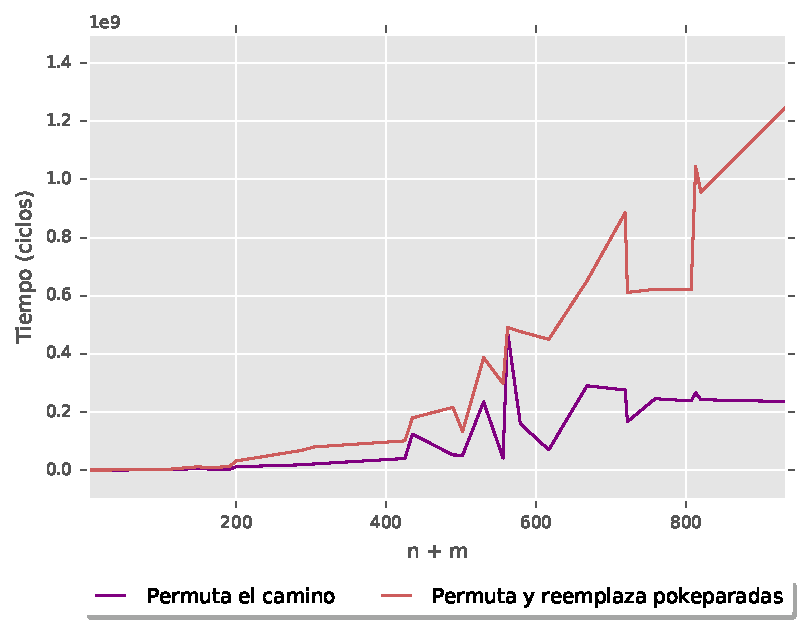
\includegraphics{../experimentacion/ej3/expAleat_cantNodos_tiempo.pdf}
    \caption{Tiempo en funci\'on de la cantidad de nodos para ambas vecindades usando instancias aleatorias.}
    \label{fig:expAleat_cantNodos_tiempo}
  \end{center}
\end{figure}

En la figura \ref{fig:expAleat_cantNodos_tiempo} podemos apreciar la relaci\'on entre la cantidad de nodos y el tiempo de ejecuci\'on con instancias aleatorias. Como podr\'ia esperarse, la que m\'as demora es la que posee el mayor porcentaje de mejora, es decir, la que probablemente m\'as modificaciones realiza sobre la soluci\'on inicial.

Por \'ultimo analizamos c\'uan buenas son las soluciones obtenidas por medio de la b\'usqueda local con respecto a laa \'optimas. Medimos esta magnitud con su error relativo:

\begin{equation*}
    error\ relativo = \frac{error\ absoluto}{valor\ exacto} = \frac{valor\ medido - valor\ exacto}{valor\ exacto}
\end{equation*}

\begin{table}[H]
    \begin{center}
        \begin{tabular}{ | l | l | l | l | l | }
            \hline
            \multicolumn{1}{|c|}{}&
            \multicolumn{2}{|c|}{\textbf{Instancias aleatorias}}&
            \multicolumn{2}{|c|}{\textbf{Instancias de mejor caso}}\\
            \cline{2-5}
                        &    \textit{Vecindad I}     &    \textit{Vecindad II}    &    \textit{Vecindad I}     &    \textit{Vecindad II}    \\ \hline
            Media       &   0.100376    &   0.127016    &   0.116154    &   0.807135    \\ \hline
            Desv\'io estandar       &   0.096465    &   0.135994    &   0.148876    &   0.937515    \\ \hline
            M\'inimo    &   0.000000    &   0.000000    &   0.000000    &   0.000000    \\ \hline
            M\'aximo    &   0.280713    &   0.484252    &   0.492888    &   2.524617    \\ \hline
        \end{tabular}
    \end{center}
    \caption{Error relativo para cada vecindad con instancias aleatorias y de mejor caso.}    
    \label{table:error_relativo}
\end{table}